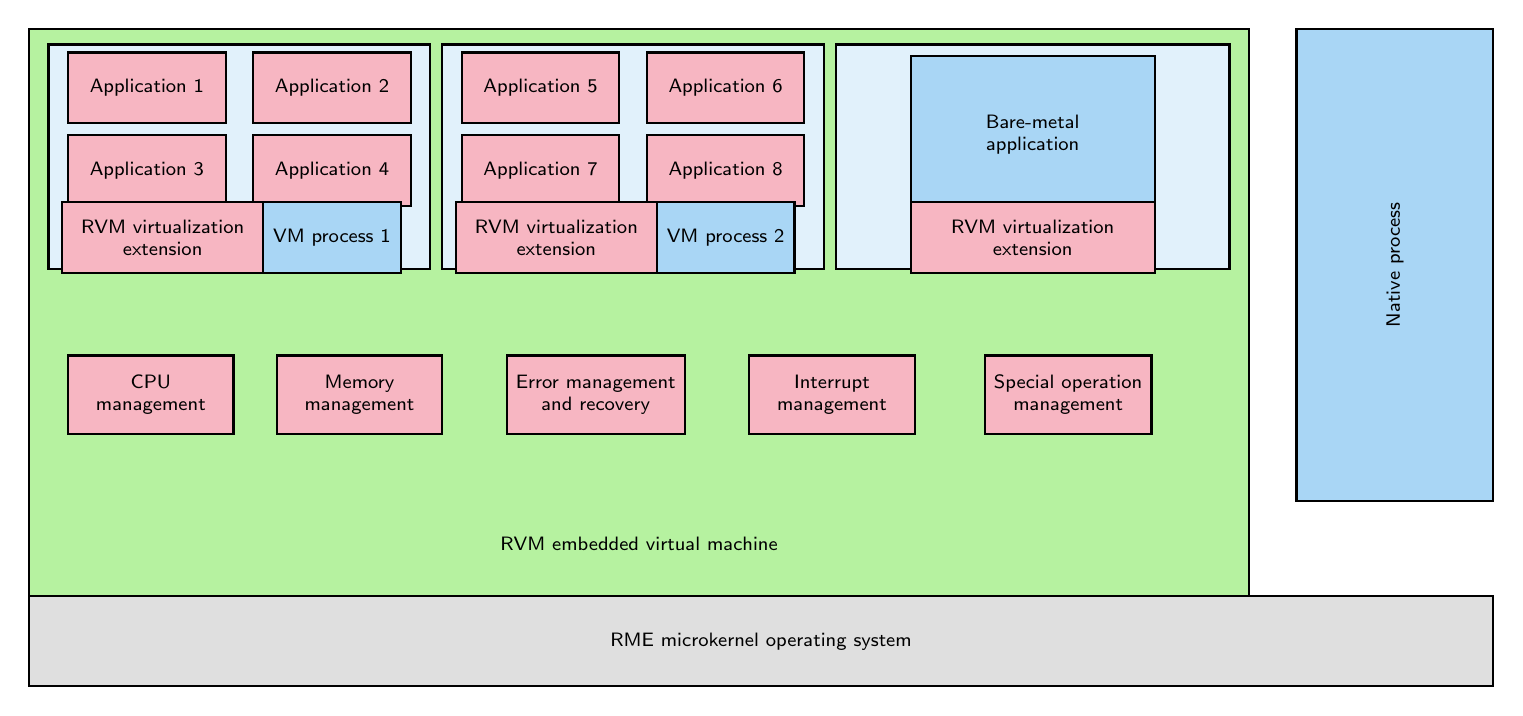
\begin{tikzpicture}[x=1cm,y=1cm,font=\sffamily\scriptsize,
    app/.style={draw,thick,fill=rvmpink,minimum width=2.0cm,minimum height=0.9cm,align=center},
    ext/.style={draw,thick,fill=rvmpink,minimum width=2.4cm,minimum height=0.9cm,align=center},
    vm/.style={draw,thick,fill=rvmblue,minimum width=2.0cm,minimum height=0.9cm,align=center},
    mgmt/.style={draw,thick,fill=rvmpink,minimum width=2.1cm,minimum height=1.0cm,align=center},
    proc/.style={draw,thick,fill=rvmblue,minimum width=2.1cm,minimum height=6.0cm,align=center}]
\definecolor{rvmgreenbg}{RGB}{182,242,160}
\definecolor{rvmpink}{RGB}{247,182,194}
\definecolor{rvmblue}{RGB}{169,214,245}
% RVM green container
\fill[rvmgreenbg] (0,0) rectangle (15.5,7.2);
\draw[thick] (0,0) rectangle (15.5,7.2);
% Three VM columns
\foreach \x/\base/\name in {0.25/1/1, 5.25/5/2} {
  \draw[thick,fill=rvmblue!35] (\x,4.15) rectangle (\x+4.85,7.0);
  \node[app] at (\x+1.25,6.45) {Application \base};
  \node[app] at (\x+3.60,6.45) {Application \the\numexpr\base+1\relax};
  \node[app] at (\x+1.25,5.40) {Application \the\numexpr\base+2\relax};
  \node[app] at (\x+3.60,5.40) {Application \the\numexpr\base+3\relax};
  \node[ext,minimum width=2.55cm] at (\x+1.45,4.55) {RVM virtualization\\extension};
  \node[vm,minimum width=1.75cm] at (\x+3.60,4.55) {VM process \name};
}
% Bare-metal column
\draw[thick,fill=rvmblue!35] (10.25,4.15) rectangle (15.25,7.0);
\node[fill=rvmblue,draw,thick,minimum width=3.1cm,minimum height=2.0cm,align=center] at (12.75,5.85) {Bare-metal\\application};
\node[ext,minimum width=3.1cm] at (12.75,4.55) {RVM virtualization\\extension};
% Management row
\node[mgmt] at (1.55,2.55) {CPU\\management};
\node[mgmt] at (4.20,2.55) {Memory\\management};
\node[mgmt] at (7.20,2.55) {Error management\\and recovery};
\node[mgmt] at (10.20,2.55) {Interrupt\\management};
\node[mgmt] at (13.20,2.55) {Special operation\\management};
\node[anchor=south] at (7.75,0.45) {RVM embedded virtual machine};
% Native process
\draw[thick,fill=rvmblue] (16.1,1.2) rectangle (18.6,7.2);
\node[rotate=90] at (17.35,4.2) {Native process};
% RME bar
\fill[gray!25] (0,-1.15) rectangle (18.6,0);
\draw[thick] (0,-1.15) rectangle (18.6,0);
\node at (9.3,-0.58) {RME microkernel operating system};
\end{tikzpicture}
